% !TEX root = ../main.tex
%
\chapter{Background}
\label{sec:background}

\section{View Synthesis}

View synthesis is a process used in computer graphics and computer vision that involves creating new, synthetic images of a scene from viewpoints that were not directly captured by a camera.
This technique leverages existing images and, often, some form of geometric information about the scene, enabling the generation of perspective-correct views at desired locations.
The goal of view synthesis is to produce realistic and accurate representations of a three-dimensional scene from novel viewpoints, enhancing applications such as virtual reality (VR), augmented reality (AR), 3D television, and film production.
The following sections provide an overview of traditional view synthesis techniques.

\paragraph{Image-Based Rendering Techniques}
Image-based rendering (IBR) techniques focus on synthesizing new views of a scene using pre-captured images, relying minimally on geometric models.
The core premise of IBR is to directly utilize the radiance information captured in these images, manipulating it to generate new viewpoints without the need for detailed 3D reconstruction.
This approach is particularly advantageous in scenarios where fast rendering is necessary or when accurate geometric data is unavailable.
IBR methods are characterized by their ability to deliver photorealistic results, as they capture lighting, shadows, and reflections true to the captured scene.
These methods, such as those using light fields or lumigraphs, excel in applications where visual realism is critical, by efficiently simulating the complexity of real-world lighting and textures \cite{buehler_unstructured_2001,chen_view_1993,debevec_modeling_1996,gortler_lumigraph_1996,levoy_light_1996}.

\paragraph{Volumetric Methods}
Volumetric rendering techniques construct a three-dimensional volume of the scene, often represented as a grid of voxels, each containing data such as color and opacity which contribute to the final image through a process akin to 3D texturing.
Unlike surface-based modeling which requires explicit surfaces, volumetric methods fill the entire data space, allowing for the handling of complex phenomena like fog, clouds, and fire, which do not have clear boundaries.
This approach is advantageous when the scene involves intricate details and volumetric phenomena that traditional polygon-based rendering might struggle to capture accurately.
Volumetric methods often use techniques like voxel coloring to integrate multiple images into a cohesive 3D model. \cite{curless_volumetric_1996,seitz_photorealistic_1999}.

\section{Neural Approaches to View Synthesis}
Neural approaches to view synthesis have significantly advanced the capabilities of generating realistic views from sparse data.
These methods integrate deep learning techniques to enhance the synthesis process, offering substantial improvements over traditional geometric and image-based methods.

\paragraph{Deep Learning for View Synthesis}
Deep learning models, particularly Convolutional Neural Networks (CNNs), are employed to predict depth and color information from sparse sets of images.
These models facilitate the synthesis of intermediate views by interpolating between captured viewpoints, efficiently handling scenarios with incomplete data where traditional methods struggle \cite{kalantari_learning-based_2016,maxim_tatarchenko_single-view_2015,peter_hedman_deep_2019}.

\paragraph{Learning Volumetric Representations}
Recent advances in neural view synthesis have explored volumetric representations to encode three-dimensional scene information effectively.
This approach leverages deep learning to construct volumetric grids or embeddings that capture both color and spatial data, allowing for dynamic and realistic rendering of new views.
Such volumetric techniques demonstrate a significant departure from traditional modeling by providing a framework where 3D features are embedded directly into the network, enabling sophisticated scene understanding and rendering without explicit geometric reconstruction \cite{lombardi_neural_2019,sitzmann_deepvoxels_2019}.

\paragraph{Multiplane Images and Scene Representation}
Multiplane Images (MPIs) represent a neural approach to view synthesis where scenes are decomposed into layers at different depths.
Neural networks learn to create these layered representations from a limited number of views.
The learned MPIs can then be efficiently re-rendered from new perspectives using traditional graphics techniques.
This method provides a robust solution for generating photorealistic and geometrically coherent views by accommodating variations in scene complexity and handling occlusions effectively \cite{mildenhall_local_2019,penner_soft_2017,pratul_p_srinivasan_pushing_2019,tao_zhou_stereo_2018}.

\paragraph{End-to-End Learning}
End-to-end learning with deep neural networks has significantly simplified the view synthesis process by enabling a single network to handle multiple synthesis tasks concurrently.
This approach reduces the complexity and potential failure points associated with multi-stage synthesis methods.
By training on large datasets of posed imagery, these networks learn complex mappings from input images to synthesized views, efficiently handling challenging scenarios \cite{chen_photographic_2017,flynn_deep_2016}.


\section{Neural Radiance Fields for View Synthesis}

Neural Radiance Fields (NeRF) offer a novel approach to view synthesis that significantly advances previous techniques. Utilizing a fully connected deep neural network, NeRF optimizes a continuous volumetric scene function from a sparse set of input views \cite{mildenhall_nerf_2021}. This method diverges from traditional discrete representations like voxel grids or mesh geometries, employing a more fluid and detailed scene representation.

\paragraph{Implementation}
NeRF synthesizes views by querying 5D coordinate space—comprising spatial locations \((x, y, z)\) and viewing directions \((\theta, \phi)\) along camera rays (a). Classic volume rendering techniques are then applied to convert the output densities and colors into images. At the heart of this process is a Multilayer Perceptron (MLP), a type of neural network characterized by layers of interconnected nodes which process input data sequentially from input to output. The MLP in NeRF takes sampled 3D points and corresponding viewing directions as input and outputs the color and volume density (b). This output is then composited into a 2D image using volume rendering techniques (c). Because this rendering function is differentiable, NeRF uses gradient descent to minimize the difference between synthesized images and observed ground truth, optimizing the neural representation of the scene (d). \fref{fig:nerf-overview}

\begin{figure}[h!]
  \centering
  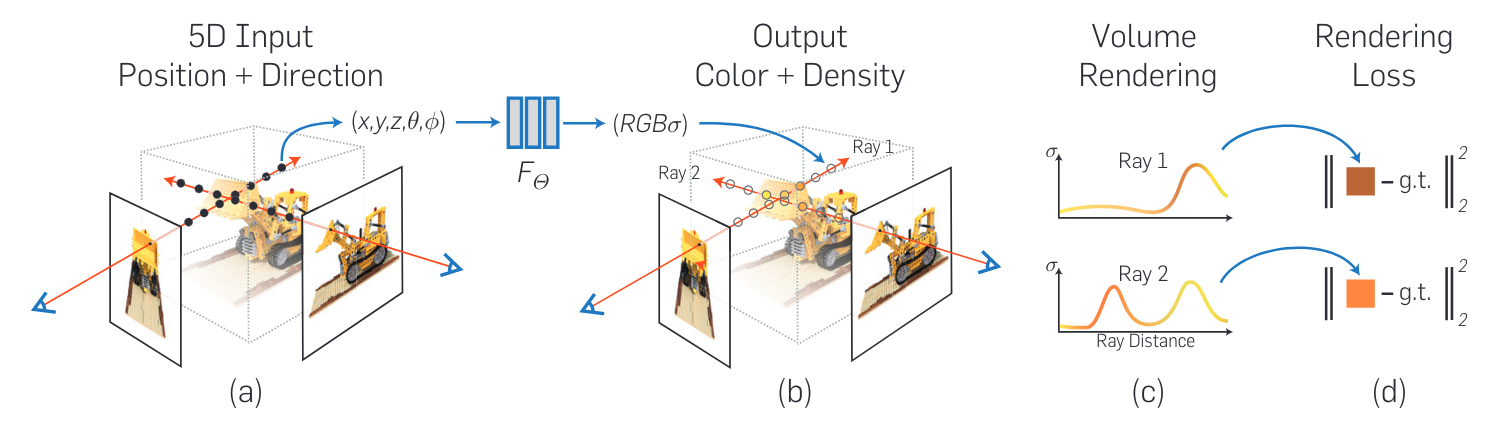
\includegraphics[width=\textwidth]{figures/bg-nerf.png}
  \caption{Overview of the NeRF scene representation and rendering procedure, illustrating the stages of sampling, neural processing, and image composition.}
  \label{fig:nerf-overview}
\end{figure}

\paragraph{Advantages of NeRF}
Compared to the methodologies discussed above, NeRF presents several advantages. It surpasses the capabilities of mesh and voxel-based methods in rendering high-resolution details and handling intricate geometries and material properties. The continuous volumetric representation is not only capable of producing more photorealistic images but also remains highly efficient in memory usage. This efficiency facilitates handling complex real-world scenes without the prohibitive storage and computation costs associated with traditional 3D representations.

In conclusion, NeRF's innovative use of neural networks for scene representation sets a new standard for photorealistic view synthesis, delivering high-quality results that are both computationally efficient and visually impressive.
